\section{Tomographie}\label{k4.2.comptomo.ct}
\sectionauthor{Aaron Gschwendt, Finja Hoffmann}

Die Tomographie ist ein bildgebendes Verfahren, in dem ein Objekt schichtweise untersucht wird. Um diese Schichten zu vermessen, beobachtet man Strahlen, die das Objekt schneiden und auf einer Ebene liegen. Die Menge an Licht, die auf der Strecke absorbiet wurde, entspricht dem Linienintegral:

$$d=\int_{\Gamma}{}s(p)dp(\gamma)$$

$s$ ist eine unbekannte Funktion, die jedem Punkt im Raum eine optische Dichte zuordnet. $d$ ist das Linienintegral von $s(p)$ entlang dem Pfad $\gamma$. $d$ entspricht der Menge an Licht, die zwischen dem Sender und dem Empfänger absorbiert wird und wird experimentell bestimmt.

Gesucht ist die Funktion $s$, diese lässt sich jedoch nicht analytisch bestimmen. Kennt man aber $d$ von genug Linien in $s$, kann man mithilfe des Satzes von Bayes mit hoher Auflösung und Sicherheit $s$ bestimmen.

\subsection{Staubtomographie}

In der Astronomie wird die Tomographie z.B. verwendet, um die Form von kosmischen Wolken zu ermitteln. Dafür werden Sterne, deren absolute Helligkeit und Distanz bekannt ist beobachtet. Man vergleicht ihre scheinbare Helligkeit mit der zu erwartende Helligkeit und ermittelt so $d$ für alle Strecken zwischen der Erde und den beobachteten Sternen. $d$ entspricht in dem Fall die Menge an Staub zwischen dem Stern und der Erde. Aus vielen (Distanz, Helligkeit)-Paaren kann man $s$ lernen und Aussagen über die dichte-Verteilung und Form der Wolke treffen.

\subsection{Computertomographie}\label{k4.2.comptomo}

Häufig verwendet wird die Tomographie auch in der Medizin, bekannt als Computertomographie(CT).

Bei herkömmlichen Röntgenuntersuchungen wird Röntgenstrahlung durch das abzubildende Objekt auf einen Röntgenfilm oder einer Sensorplatte geleitet. Das 3d-Objekt wird dabei auf eine 2d-Fläche projiziert. Der Nachteil dieser Methode ist, dass sich Teile vom Objekt überlagern können und nicht erkannt werden kann, ob es sich um ein Objekt mit hoher Absorption oder mehrer Objekte mit geringer Absorption handelt.

Beim CT drehen sich im $180^\circ$ Winkel eine Röntgenröhre und Detektor um den Patienten und nehmen dabei in kleinen Abständen Messpunkte auf. Dies wird für mehrere Schichten entlang des zu untersuchenden Körperteils ausgeführt. Der Röntgenstrahl und Detektor ist so breit, dass bei jedem Messpunkt die ganze Breite des Körperteils in einem Streifen ergriffen wird.

\begin{figure}
 \centering
 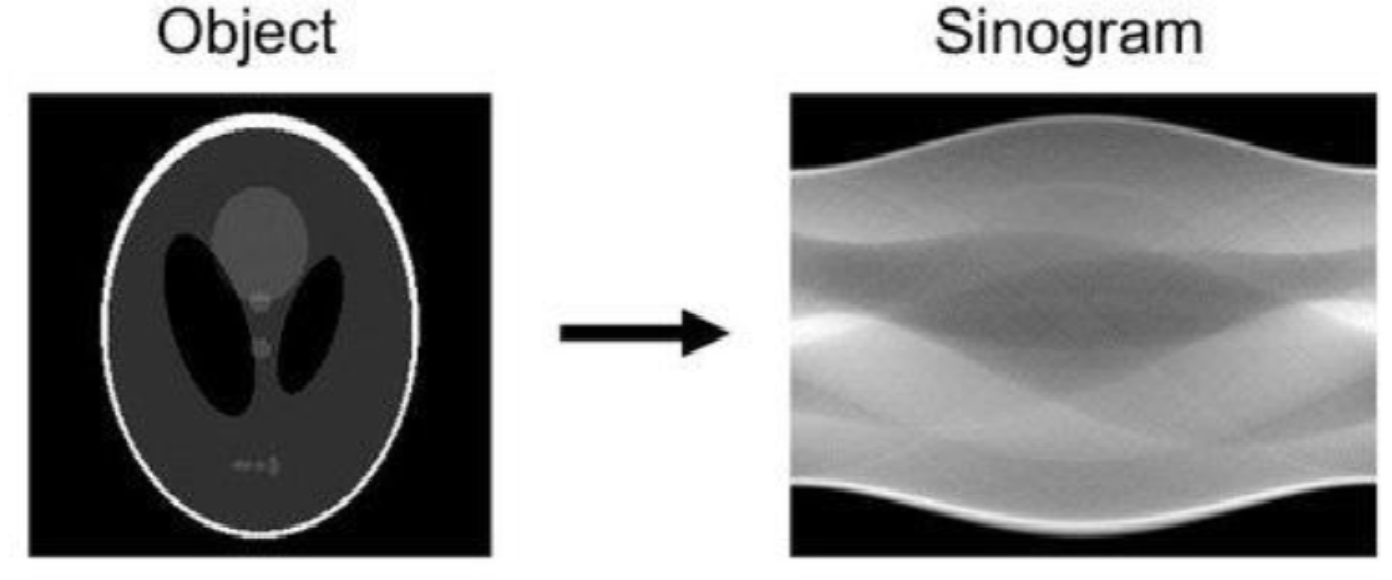
\includegraphics[width=0.4\textwidth]{k4.2/backprojektion.png}
 \caption{Abbildung eines Objektes als Sinogram}
 \label{k4.2.tomo.ct.bp}
\end{figure}

Daraus entsteht für jede Schicht ein Sinogram \cref{k4.2.tomo.ct.bp} bei der eine Achse (hier Y-Achse) das Absorptionsprofil und die andere (hier X-Achse) dem Winkel entspricht. Jede Stelle im Objekt bildet eine Sinuskurve; ihr Abstand vom Mittelpunkt entspricht der Amplitude und ihr Winkel im vergleich zum Startpunkt der Phasenverschiebung der Sinuskurve. Mit dem bayeschen Verfahren  kann man ein Bild von der Schicht mit hoher Genauigkeit rekonstruieren. Führt man dies für jede durch, Schicht erhält man ein 3d-Rendering des Objekts.


\subsection{CT in 3D}\label{k4.2.ct.3d}
\sectionauthor{Finja Hoffmann, Chuyang Wang}

Im Rahmen der Projektarbeit soll aus den gemessenen Daten $d$ die Funktion des Signals $s(p)$ (\emph{quantity of interest}) in Abhängigkeit von einem 3D-Punkt $p \in \mathbb{R}^3$ rekonstruiert werden, welche die Dichte eines Objekts in einem diskreten 3-dimensionalen Raum beschreibt. Generell lässt sich der Datenvektor $d \in \mathbb{R}^N$ wie folgt berechnen:

\begin{equation}
  \label{k4.2.ct.3d.datamodel}
  \begin{aligned}
    d = Rs + n,
  \end{aligned}
\end{equation}

wobei $R \in \mathbb{R}^{N \times M}$ die \emph{Response}, $s \in \mathbb{R}^M$ das Signal und $n \in \mathbb{R}^N$ das Rauschen beschreiben. 
% TODO: ref to Wiener Filter

\subsection{Line-Of-Sight Response}\label{k4.2.ct.resp}

Angenommen, die Start- und Endpunkte der Messungen seien bereits gegeben und bilden jeweils die Strecken. Aus diesen Daten kann man die Matrix $R$ konstruieren. Anders gesagt repräsentiert $R$ die Start- und Endpunkten. Da das Signal (die Dichtenverteilung) in Form von diskreten 3D-Pixel angegeben sind, ist $R$ eine Matrix der Gewichte der gegebenen Komponenten des Signals. Als Gewichtung eines Datenwürfels gilt der euklidischen Abstand zwischen den beiden Schnittpunkten der Strecke mit den Seiten des Würfels. \textcite{k4.2.siddon} hat dafür einen effizienten Algorithmus geliefert, dessen Ansatz hier umgesetzt wird.


\subsection{Algorithmus von Siddon}\label{k4.2.ct.siddon}

Siddons Ansatz nach könnte man die Schnittpunkte einer Sichtlinie mit den x-, y- und z-Achsenebenen jeweils einzeln bestimmen und in sortierte Listen $A$, $B$ und $C$ speichern. Sei jeweils

\begin{equation}
  P_{start} = \begin{pmatrix}x_{start} \\ y_{start} \\ z_{start}\end{pmatrix}
\end{equation}

\begin{equation}
  P_{end} = \begin{pmatrix}x_{end} \\ y_{end} \\ z_{end}\end{pmatrix}
\end{equation}

Betrachtet man zunächst die x-Achsenebene. Ohne Beschränkung der Allgemeinheit sei $x_{start} < x_{end}$. Man rundet die x-Koordinate des Startpunktes in die Richtung der Strecke auf und berechnet die Differenz $x^{\ast}$. Um die y- und z-Koordinaten dieses ersten Schnittpunkts herauszufinden, muss man noch die Steigungen gegenüber dieser beiden Achsen $m_{yx} = \frac{y_{end} - y_{start}}{x_{start} - x_{end}}$ und $m_{zx} = \frac{z_{end} - z_{start}}{x_{start} - x_{end}}$ berechnen. Somit erhält man den ersten Schnittpunkt

\begin{equation}
  S_{x,0} = \begin{pmatrix}
    x_{start} + x^{\ast} \\
    y_{start} + x^{\ast} \cdot m_{yx} \\
    z_{start} + x^{\ast} \cdot m_{zx} \\
  \end{pmatrix}.
\end{equation}

Die weiteren Schnittpunkte $S_{x,i}$ kann man rekursiv konstruieren, indem man jeweils eine Einheit in die x-Richtung geht und die Änderungsrate gegenüber der y- und z-Achsen jeweils aufaddiert

\begin{equation}
  S_{x,i} = S_{x,i-1} + \begin{pmatrix}
    1 \\
    1 \cdot m_{yx} \\
    1 \cdot m_{zx} \\
  \end{pmatrix}.
\end{equation}

 Die Liste $A$ besteht aus allen Schnittpunkten $[S_{x,0}, S_{x,1}, ..., S_{x,n}]$ mit x-Ebenen. Die Listen $B$ und $C$ berechnet man analog.

Anschließend muss man die drei Listen in eine einzelne sortierte Liste $\mathbf{S}$ zusammenführen. Diese geschieht, indem man alle Schnittpunkte aus $A$, $B$ und $C$ nach den x-Koordinaten aufsteigend sortiert. Sollte $x_{start} = x_{end}$ sein, dann nutzt man die y- oder z-Achse als den Sortierschlüssel.

Hat man alle sortierten Schnittpunkte, so kann man auch die Gewichtungen, i.e. die Abstände zwischen den jeweiligen Punkten, einfach berechnen. Jede dieser Gewichtungen wird einem 3D-Pixel zugeordnet, durch den diese Teilstrecke durchdringt. Für diese Sichtlinie kann dann ein Zeilenvektor $r_i$ erstellt werden, welcher diese Zuordnung von Gewichtungen speichert. Man beobachte, dass jede Sichtlinie nur wenige Pixeln im 3D-Raum durchgeht. Die meisten Gewichte für die diskretisierte Dichtenverteilung entlang einer Sichtlinie sind null.


\subsection{Walnuss CT-Messdaten}\label{k4.2.ct.walnuss}
\sectionauthor{Leo Bergmann, Cedric Balzer}
\begin{figure}
	\centering
	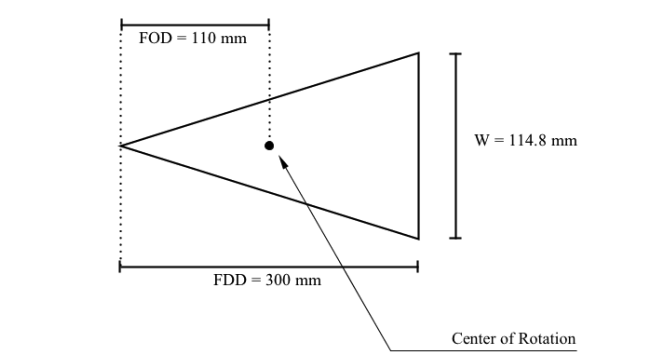
\includegraphics[width=0.7\textwidth]{k4.2/geometry.png}
	\caption{Aufbau des Versuchs mit dessen Geometrie aus \textcite{k4.2.hamalainen2015tomographic}.
	FOD steht für \enquote{Focus-to-object} distance, FDD für \enquote{Focus-to-detector} distance und W für die Breite des Detektors.
	}
	\label{k4.2.fig.geo}
\end{figure}

Das Ziel des Projekts ist es ein Bild einer Walnuss, anhand von CT-Scandaten (siehe \cref{k4.2.comptomo}), zu rekonstruieren. Die Herausforderung besteht darin die Unsicherheit in der DIchteverteilung des zu vermessenden Objekts zu quantifiziern. Aus ein Bayes'schen Perspektive (siehe \cref{k4.2.bayes}) quantifiziert der Posterior die Unsicherheit. Die präzise Beschreibung ist bei medizinischer Bildgebung wichtig.
Die Daten, auf welchen unser Projekt beruht, enthalten Sinogramm und Schichtaufnahme einer Walnuss, welche in \verb|.mat|-Dateien gespeichert sind \parencite{k4.2.hamalainen2015tomographic}.
In dem Versuch wurde eine Walnuss zwischen eine punktförmige Strahlungsquelle und einen flachen Schirm positioniert (\cref{k4.2.fig.geo}). Nach jeder Messung wurde die Nuss um 3° gegen den Uhrzeigersinn gedreht.
Insgesamt wurden 120 Messungen durchgeführt. Diese Daten wurden auf 328 Pixel herunterskaliert und in einer Matrix \verb|m| gespeichert.
Damit das Sinogramm in ein Bild der Dichteverteilung zurückprojeziert werden kann sind alle Start- und Endpunkte der Sichtline notwendig. Diese errechnen sich aus der Position der Quelle und der Position der einzelnen Pixel des Screens.\\


\begin{figure}
	\centering
	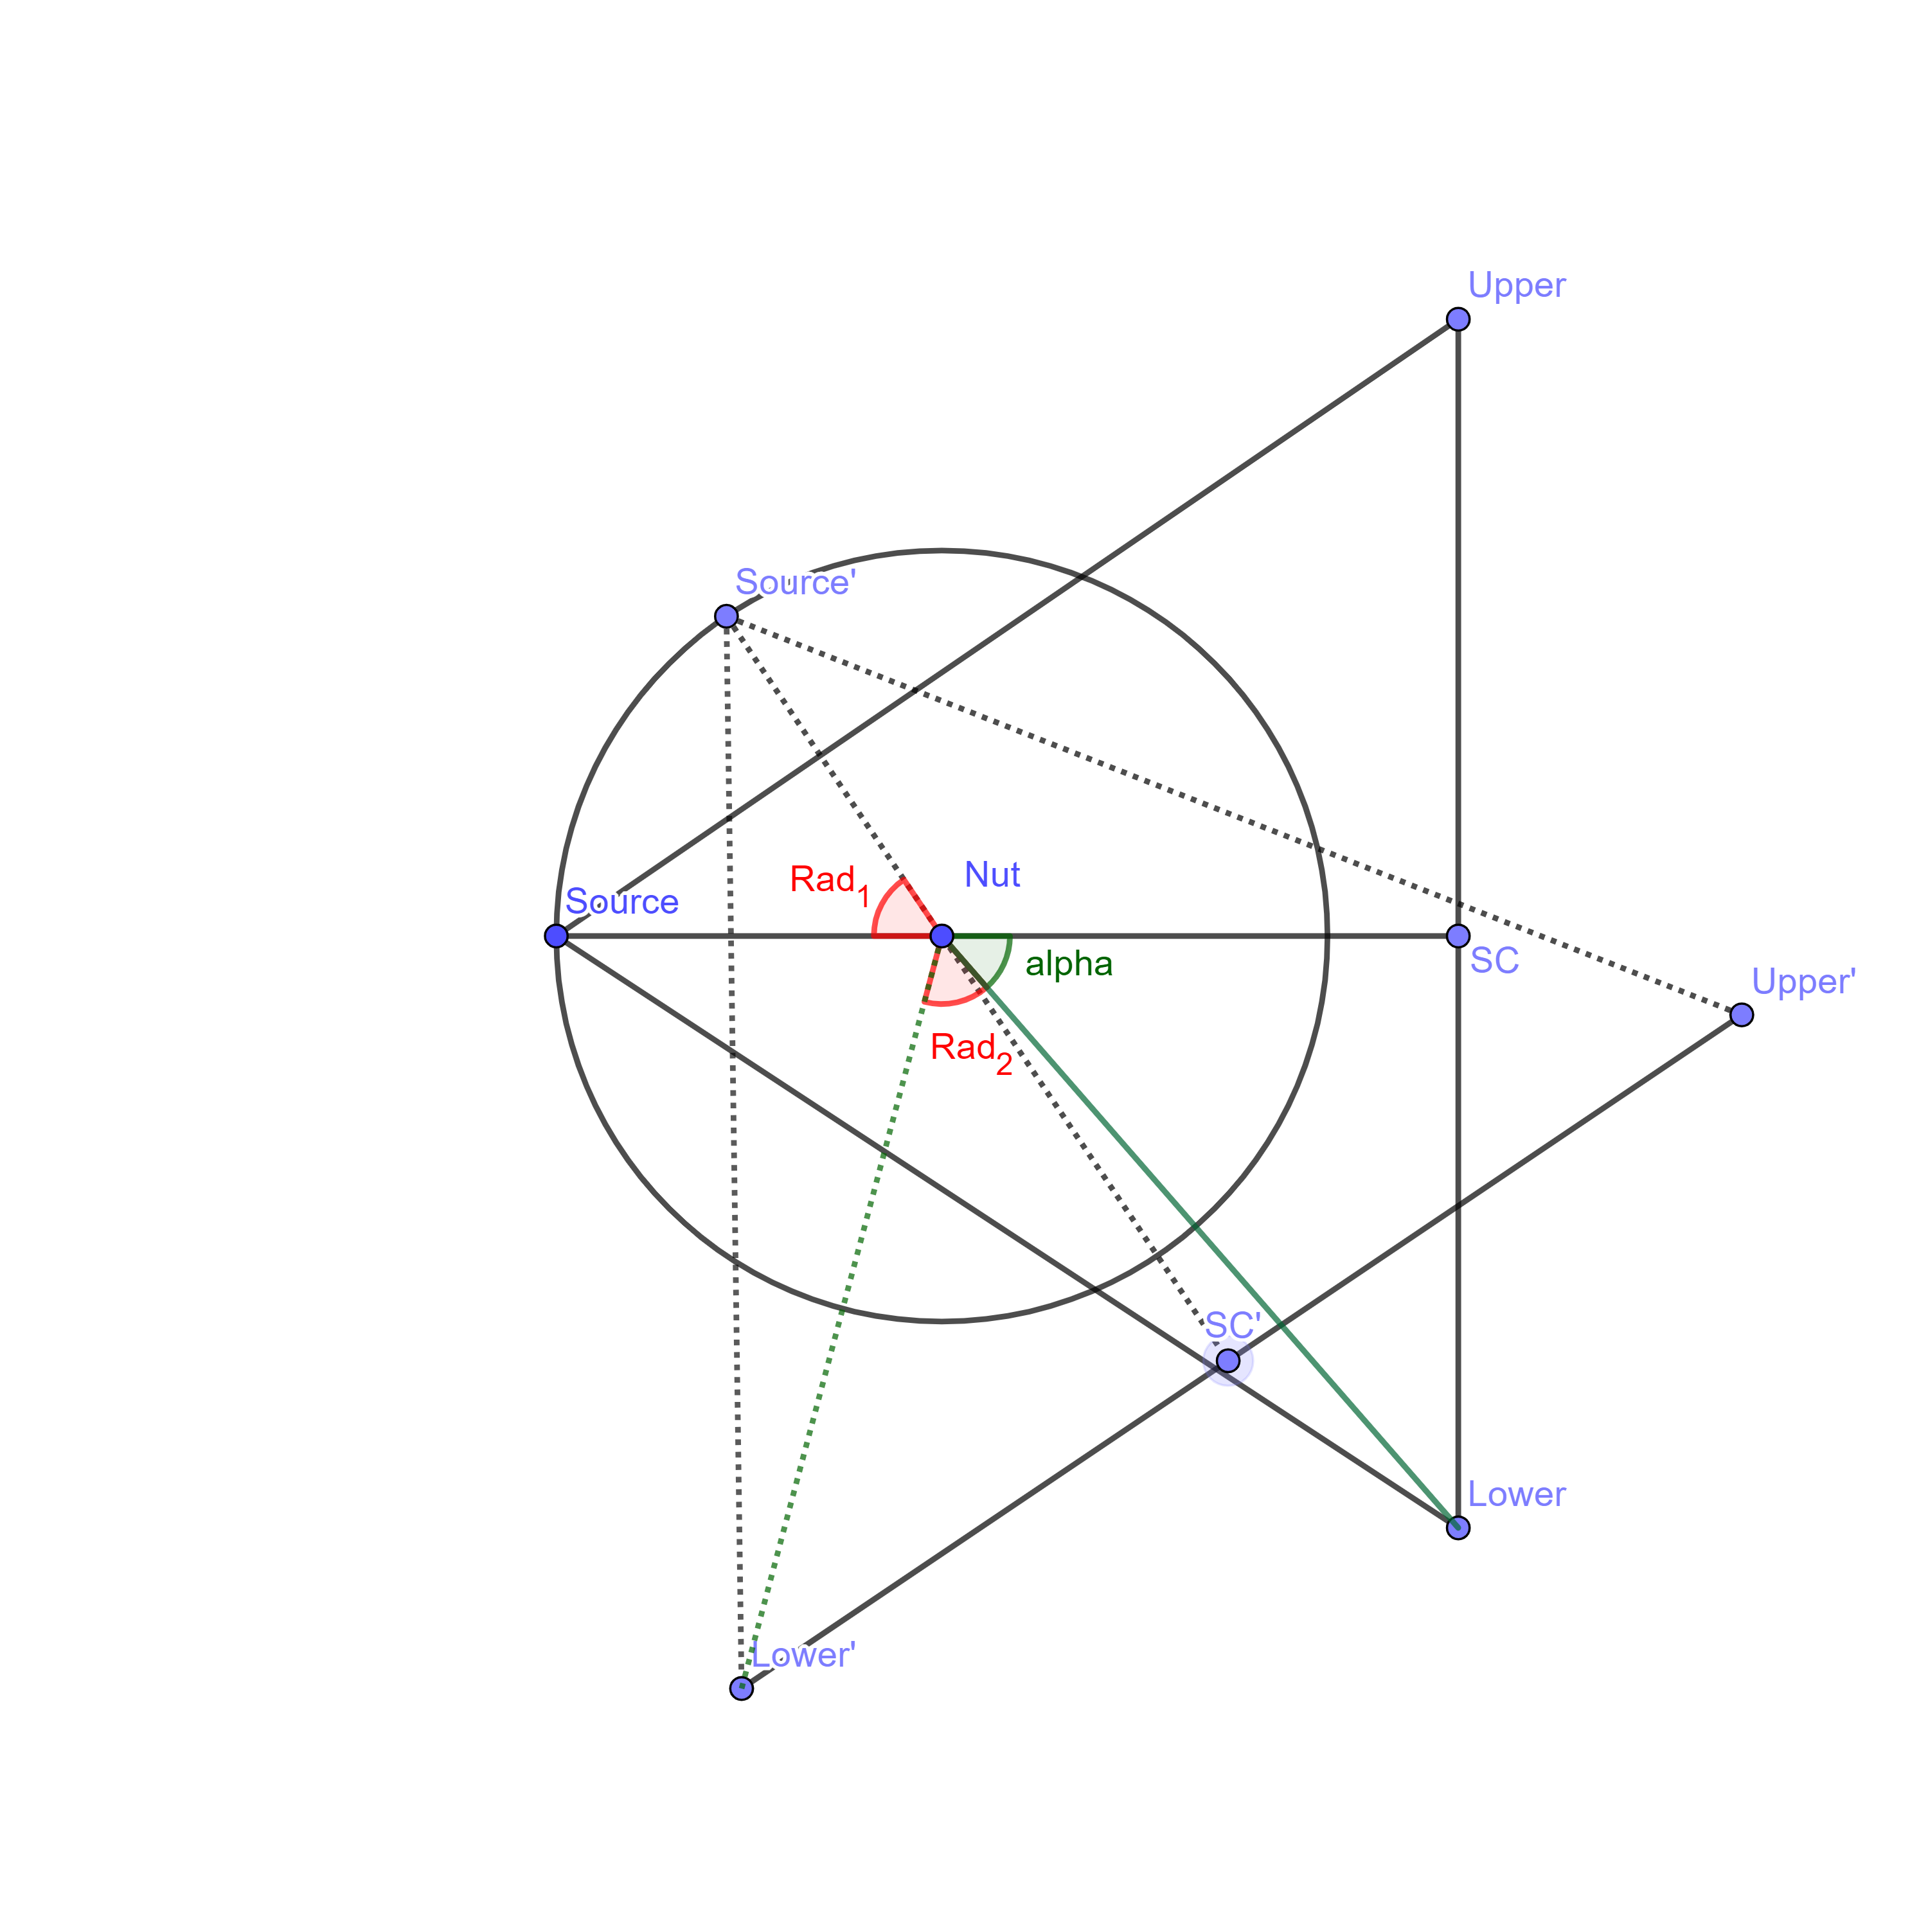
\includegraphics[width=0.4\textwidth]{k4.2/versuchsaufbau-skizze.png}
	\caption{Versuchsaufbau skizziert. \\
	$S$ steht für die Startpunkt der Strahlenquelle, $N$ ist die gescannte Walnuss, $U$ repräsentiert die obere äußere Grenzen des Detektors und $L$ respektive die Untere, $\delta$ steht für den Laufwinkel welcher in 3° Schritten erhöht wird, $\alpha$ für den Winkel zwischen X-Achse und $L$. $C$ ist der Mittelpunkt des Detektors.
	}
	\label{k4.2.fig.skizze}
\end{figure}

Anstelle einer Drehung der Nuss gegen den Uhrzeigersinn betrachten wir, äquivalent dazu, eine kreisförmigen Rotation des Detektors (Screen) und der Strahlungsquelle (S) um die Walnuss (N) (siehe \cref{k4.2.fig.skizze}). Es bieten sich Polarkoordinaten an, um die Position der Quelle und des Detektors relativ zu Walnuss zu bestimmen, jedoch müssen alle Punkte für die Weiterverarbeitung im kartesischen Koordinatensystem angegeben. Da die Winkel und Abstandsmaße in Bezug auf die Walnuss angegeben sind, wird diese als Koordinatenursprung definiert. Ausgehend davon wird die Quelle zunächst an die Stelle $\begin{pmatrix}-110\\ 0 \end{pmatrix}$   gelegt (siehe \cref{k4.2.fig.geo}, \cref{k4.2.fig.skizze}). Dadurch wird die Startposition des Detektors festgelegt, der durch seinen Anfang ($U$) an Stelle $\begin{pmatrix}190\\ 57.4 \end{pmatrix}$ und seinen Endpunkt ($L$) an Stelle $\begin{pmatrix}190\\ -57.4 \end{pmatrix}$ bestimmt wird. 
$S‘$ entspricht $S$ nach einer Drehung der Quelle und des Detektors um den Winkel $\delta$. Der Abstand zwischen $S‘$ und $\mathrm{N}$ ist dabei immer 110 mm. Der Versuchsaufbau kann somit als Einheitskreis mit Mittelpunkt $N$ interpretiert werden, der um den Faktor 110 mm gestreckt wurde. Dadurch ist im kartesischen Koordinatensystem die horizontale Koordinaten-Komponente von $S‘$ gleich $\cos(\delta) * 110\text{ mm}$ und die vertikale Komponente gleich $\sin(\delta) * 110\text{ mm}$.
Der Winkel $\sphericalangle U-N-L$ hat eine Größe von etwa 34°, somit hat der Winkel $\alpha = \sphericalangle L-N-C$ eine Größe von 17°. Der Abstand von $N$ zu $L$ kann mithilfe des Satzes von Pythagoras berechnet werden $d = \sqrt{(300\text{ mm} - 110\text{ mm})^2+(114.8\text{ mm}/2)^2} = 198.48\text{ mm}$.
Der Winkel $\alpha$ addiert mit $\delta$ ergibt zusammen mit der Länge $d$ die Koordinaten $L$ im Polarkoordinaten. Um $U‘$ zu berechnen muss $\alpha$ von $\delta$ subtrahiert werden. Die entsprechenden kartesischen Koordinaten erhalten wir nun auf gleiche Weise bei $S‘$. Die restlichen 328 Pixelpositionen des Detektors sind gleichmäßige auf der Verbindumgsstecke zwischen $U$ und $L$ verteilt.
Mit den erhaltenen Start- und Endpunkten können die Helligkeitswerte zum Raum der Dichteverteilung zurückprojiziert werden.
Die erhaltenen Start und Endpunkte, in Kombination mit den im Datenset gelieferten Helligkeitswerten kann nun in ein vollständing rüchprojeziertes CT Schichtbild verwandelt werden.


\subsection{Rekonstruktion des Signals}
\sectionauthor{Chuyang Wang}

Das Ziel der Computertomographie ist, das Signal aus den gemessenen Daten zu berechnen. Mit Bayes' Formel aus \cref{k4.2.bayes} kann man den gesuchten Posterior $P(s|d)$ mit der Likelihood $P(d|s)$ und Prior $P(s)$ wie folgt konstruieren:

\begin{equation}
  P(s|d) \propto P(d|s)P(s)\ .
\end{equation}

Für die Likelihood gilt:

\begin{equation}
  \begin{aligned}
    && P(d|s) &= \int P(d,n|s) \,dn  \\
    &&  &= \int P(d|s,n) P(n|s) \,dn \\
    && &= \int P(d|s,n) P(n) \,dn \ .
  \end{aligned}
\end{equation}

Es gilt außerdem das Datenmodell \cref{k4.2.ct.3d.datamodel}. Da bei $P(d|s,n)$ $s$ und $n$ bekannt sind, ist auch $d$ fest. Eine empirische Analyse der Daten hat gezeigt, dass das Rauschen $P(n) = \mathcal{G}(n,N)$ normalverteilt ist. Für normal verteiltes Rauschen lässt sich zeigen, dass folgende Gleichung gilt:

% delta Distribution
\begin{equation}
  \begin{aligned}
    &\Rightarrow& P(d|s) &= P_n(n-(d-Rs)) \\ 
    && &= \mathcal{G}(d-Rs,N) \ .
  \end{aligned}
\end{equation}

Die Daten $d$ wurden im Experiment gemessen (vgl. \cref{k4.2.ct.walnuss}). Die Response $R$ beschreibt das Experiment (vgl. \cref{k4.2.ct.resp}) und kann vorberechnet werden. Um den Posterior zu bestimmen, muss man die Annahmen für das Signal $s$ formulieren. Man wählt dafür ein hierarchisches Modell (vgl. \cref{k4.2.hiera}). Dabei nutzt man aus, dass $s$ positiv sein muss. Also kann man $s$ mit einer Log-Normalverteilung beschreiben. 

Um den Posterior $P(s|d) = \frac{P(d|s)P(s)}{P(d)}$ zu berechnen, benötigt man auch die Evidenz als Normierungsfaktor. Diese ist jedoch computational zu teuer. Man nutzt die Kullback-Leibler-Divergenz (vgl. \cref{k4.2.kldiv}), um den Posterior mit $P_a$ anzunähern $\mathrm{KL}(P_a,P)$. 


\subsection{Endergebnis}

Implementiert man das obige Verfahren, so erhält man am Ende eine approximative Wahrscheinlichkeitsverteilung für das Signal $P(s|d)$ mit gegebenen Daten $d$. Die \cref{k4.2.fig.ct.mean} zeigt den Erwartungswert über mehrere Stichproben der approximativen Verteilung. An der Standardabweichung \cref{k4.2.fig.ct.std} erkennt man, dass die absolute Unsicherheit an den Stellen der Walnuss höher ist, an denen besonders viel Walnuss-Masse liegt. 

\begin{figure}
  \centering
  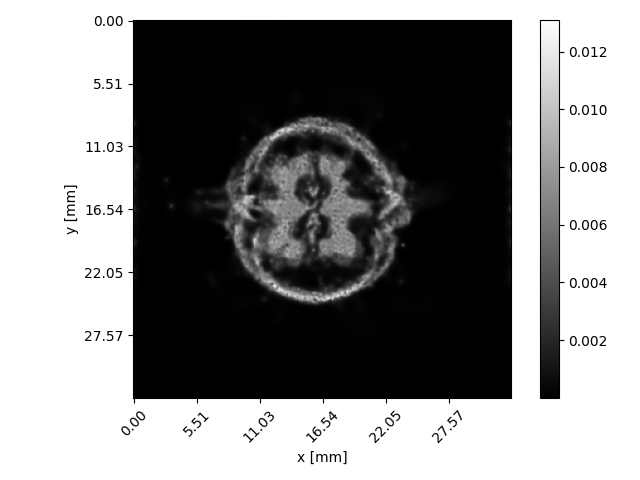
\includegraphics[width=0.6\textwidth]{k4.2/ct-walnuss-mean.png}
  \caption{Erwartungswert des Posteriors.}
  \label{k4.2.fig.ct.mean}
\end{figure}

\begin{figure}
  \centering
  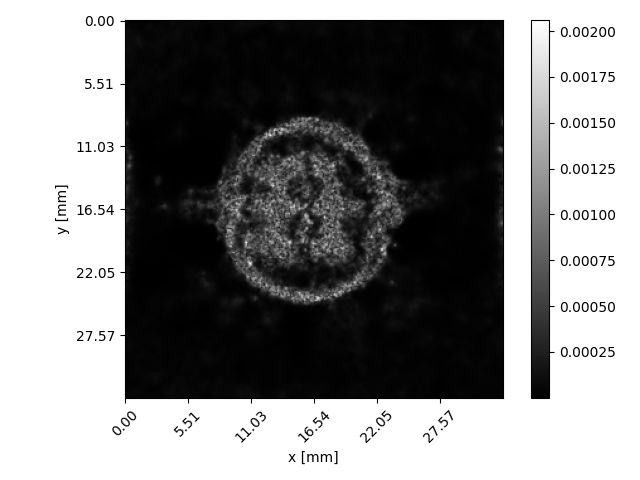
\includegraphics[width=0.6\textwidth]{k4.2/ct-walnuss-std.png}
  \caption{Standardabweichung des Posteriors.}
  \label{k4.2.fig.ct.std}
\end{figure}

An manchen Stellen wie z.B. $(10|17)$ und $(22|20)$ der \cref{k4.2.fig.ct.mean} sind unscharfe Kanten sowie teilweise Rauschen zu erkennen. Diese Fehler bei dem Modell könnten daran liegen, dass das Optimum von der Kullback-Leibler-Divergenz nur annäherungsweise erreicht ist. Darüber hinaus ist das Modell eventuell zu stark vereinfachend für die Beschreibung der Walnuss. 
